% Options for packages loaded elsewhere
\PassOptionsToPackage{unicode}{hyperref}
\PassOptionsToPackage{hyphens}{url}
\PassOptionsToPackage{dvipsnames,svgnames,x11names}{xcolor}
%
\documentclass[
  letterpaper,
  DIV=11,
  numbers=noendperiod]{scrartcl}

\usepackage{amsmath,amssymb}
\usepackage{iftex}
\ifPDFTeX
  \usepackage[T1]{fontenc}
  \usepackage[utf8]{inputenc}
  \usepackage{textcomp} % provide euro and other symbols
\else % if luatex or xetex
  \usepackage{unicode-math}
  \defaultfontfeatures{Scale=MatchLowercase}
  \defaultfontfeatures[\rmfamily]{Ligatures=TeX,Scale=1}
\fi
\usepackage{lmodern}
\ifPDFTeX\else  
    % xetex/luatex font selection
\fi
% Use upquote if available, for straight quotes in verbatim environments
\IfFileExists{upquote.sty}{\usepackage{upquote}}{}
\IfFileExists{microtype.sty}{% use microtype if available
  \usepackage[]{microtype}
  \UseMicrotypeSet[protrusion]{basicmath} % disable protrusion for tt fonts
}{}
\makeatletter
\@ifundefined{KOMAClassName}{% if non-KOMA class
  \IfFileExists{parskip.sty}{%
    \usepackage{parskip}
  }{% else
    \setlength{\parindent}{0pt}
    \setlength{\parskip}{6pt plus 2pt minus 1pt}}
}{% if KOMA class
  \KOMAoptions{parskip=half}}
\makeatother
\usepackage{xcolor}
\usepackage{soul}
\setlength{\emergencystretch}{3em} % prevent overfull lines
\setcounter{secnumdepth}{-\maxdimen} % remove section numbering
% Make \paragraph and \subparagraph free-standing
\ifx\paragraph\undefined\else
  \let\oldparagraph\paragraph
  \renewcommand{\paragraph}[1]{\oldparagraph{#1}\mbox{}}
\fi
\ifx\subparagraph\undefined\else
  \let\oldsubparagraph\subparagraph
  \renewcommand{\subparagraph}[1]{\oldsubparagraph{#1}\mbox{}}
\fi

\usepackage{color}
\usepackage{fancyvrb}
\newcommand{\VerbBar}{|}
\newcommand{\VERB}{\Verb[commandchars=\\\{\}]}
\DefineVerbatimEnvironment{Highlighting}{Verbatim}{commandchars=\\\{\}}
% Add ',fontsize=\small' for more characters per line
\usepackage{framed}
\definecolor{shadecolor}{RGB}{241,243,245}
\newenvironment{Shaded}{\begin{snugshade}}{\end{snugshade}}
\newcommand{\AlertTok}[1]{\textcolor[rgb]{0.68,0.00,0.00}{#1}}
\newcommand{\AnnotationTok}[1]{\textcolor[rgb]{0.37,0.37,0.37}{#1}}
\newcommand{\AttributeTok}[1]{\textcolor[rgb]{0.40,0.45,0.13}{#1}}
\newcommand{\BaseNTok}[1]{\textcolor[rgb]{0.68,0.00,0.00}{#1}}
\newcommand{\BuiltInTok}[1]{\textcolor[rgb]{0.00,0.23,0.31}{#1}}
\newcommand{\CharTok}[1]{\textcolor[rgb]{0.13,0.47,0.30}{#1}}
\newcommand{\CommentTok}[1]{\textcolor[rgb]{0.37,0.37,0.37}{#1}}
\newcommand{\CommentVarTok}[1]{\textcolor[rgb]{0.37,0.37,0.37}{\textit{#1}}}
\newcommand{\ConstantTok}[1]{\textcolor[rgb]{0.56,0.35,0.01}{#1}}
\newcommand{\ControlFlowTok}[1]{\textcolor[rgb]{0.00,0.23,0.31}{#1}}
\newcommand{\DataTypeTok}[1]{\textcolor[rgb]{0.68,0.00,0.00}{#1}}
\newcommand{\DecValTok}[1]{\textcolor[rgb]{0.68,0.00,0.00}{#1}}
\newcommand{\DocumentationTok}[1]{\textcolor[rgb]{0.37,0.37,0.37}{\textit{#1}}}
\newcommand{\ErrorTok}[1]{\textcolor[rgb]{0.68,0.00,0.00}{#1}}
\newcommand{\ExtensionTok}[1]{\textcolor[rgb]{0.00,0.23,0.31}{#1}}
\newcommand{\FloatTok}[1]{\textcolor[rgb]{0.68,0.00,0.00}{#1}}
\newcommand{\FunctionTok}[1]{\textcolor[rgb]{0.28,0.35,0.67}{#1}}
\newcommand{\ImportTok}[1]{\textcolor[rgb]{0.00,0.46,0.62}{#1}}
\newcommand{\InformationTok}[1]{\textcolor[rgb]{0.37,0.37,0.37}{#1}}
\newcommand{\KeywordTok}[1]{\textcolor[rgb]{0.00,0.23,0.31}{#1}}
\newcommand{\NormalTok}[1]{\textcolor[rgb]{0.00,0.23,0.31}{#1}}
\newcommand{\OperatorTok}[1]{\textcolor[rgb]{0.37,0.37,0.37}{#1}}
\newcommand{\OtherTok}[1]{\textcolor[rgb]{0.00,0.23,0.31}{#1}}
\newcommand{\PreprocessorTok}[1]{\textcolor[rgb]{0.68,0.00,0.00}{#1}}
\newcommand{\RegionMarkerTok}[1]{\textcolor[rgb]{0.00,0.23,0.31}{#1}}
\newcommand{\SpecialCharTok}[1]{\textcolor[rgb]{0.37,0.37,0.37}{#1}}
\newcommand{\SpecialStringTok}[1]{\textcolor[rgb]{0.13,0.47,0.30}{#1}}
\newcommand{\StringTok}[1]{\textcolor[rgb]{0.13,0.47,0.30}{#1}}
\newcommand{\VariableTok}[1]{\textcolor[rgb]{0.07,0.07,0.07}{#1}}
\newcommand{\VerbatimStringTok}[1]{\textcolor[rgb]{0.13,0.47,0.30}{#1}}
\newcommand{\WarningTok}[1]{\textcolor[rgb]{0.37,0.37,0.37}{\textit{#1}}}

\providecommand{\tightlist}{%
  \setlength{\itemsep}{0pt}\setlength{\parskip}{0pt}}\usepackage{longtable,booktabs,array}
\usepackage{calc} % for calculating minipage widths
% Correct order of tables after \paragraph or \subparagraph
\usepackage{etoolbox}
\makeatletter
\patchcmd\longtable{\par}{\if@noskipsec\mbox{}\fi\par}{}{}
\makeatother
% Allow footnotes in longtable head/foot
\IfFileExists{footnotehyper.sty}{\usepackage{footnotehyper}}{\usepackage{footnote}}
\makesavenoteenv{longtable}
\usepackage{graphicx}
\makeatletter
\def\maxwidth{\ifdim\Gin@nat@width>\linewidth\linewidth\else\Gin@nat@width\fi}
\def\maxheight{\ifdim\Gin@nat@height>\textheight\textheight\else\Gin@nat@height\fi}
\makeatother
% Scale images if necessary, so that they will not overflow the page
% margins by default, and it is still possible to overwrite the defaults
% using explicit options in \includegraphics[width, height, ...]{}
\setkeys{Gin}{width=\maxwidth,height=\maxheight,keepaspectratio}
% Set default figure placement to htbp
\makeatletter
\def\fps@figure{htbp}
\makeatother

\KOMAoption{captions}{tableheading}
\makeatletter
\makeatother
\makeatletter
\makeatother
\makeatletter
\@ifpackageloaded{caption}{}{\usepackage{caption}}
\AtBeginDocument{%
\ifdefined\contentsname
  \renewcommand*\contentsname{Table of contents}
\else
  \newcommand\contentsname{Table of contents}
\fi
\ifdefined\listfigurename
  \renewcommand*\listfigurename{List of Figures}
\else
  \newcommand\listfigurename{List of Figures}
\fi
\ifdefined\listtablename
  \renewcommand*\listtablename{List of Tables}
\else
  \newcommand\listtablename{List of Tables}
\fi
\ifdefined\figurename
  \renewcommand*\figurename{Figure}
\else
  \newcommand\figurename{Figure}
\fi
\ifdefined\tablename
  \renewcommand*\tablename{Table}
\else
  \newcommand\tablename{Table}
\fi
}
\@ifpackageloaded{float}{}{\usepackage{float}}
\floatstyle{ruled}
\@ifundefined{c@chapter}{\newfloat{codelisting}{h}{lop}}{\newfloat{codelisting}{h}{lop}[chapter]}
\floatname{codelisting}{Listing}
\newcommand*\listoflistings{\listof{codelisting}{List of Listings}}
\makeatother
\makeatletter
\@ifpackageloaded{caption}{}{\usepackage{caption}}
\@ifpackageloaded{subcaption}{}{\usepackage{subcaption}}
\makeatother
\makeatletter
\@ifpackageloaded{tcolorbox}{}{\usepackage[skins,breakable]{tcolorbox}}
\makeatother
\makeatletter
\@ifundefined{shadecolor}{\definecolor{shadecolor}{rgb}{.97, .97, .97}}
\makeatother
\makeatletter
\makeatother
\makeatletter
\makeatother
\ifLuaTeX
  \usepackage{selnolig}  % disable illegal ligatures
\fi
\IfFileExists{bookmark.sty}{\usepackage{bookmark}}{\usepackage{hyperref}}
\IfFileExists{xurl.sty}{\usepackage{xurl}}{} % add URL line breaks if available
\urlstyle{same} % disable monospaced font for URLs
\hypersetup{
  pdftitle={Quarto Basics},
  colorlinks=true,
  linkcolor={blue},
  filecolor={Maroon},
  citecolor={Blue},
  urlcolor={Blue},
  pdfcreator={LaTeX via pandoc}}

\title{Quarto Basics}
\author{}
\date{}

\begin{document}
\maketitle
\ifdefined\Shaded\renewenvironment{Shaded}{\begin{tcolorbox}[interior hidden, borderline west={3pt}{0pt}{shadecolor}, sharp corners, frame hidden, breakable, enhanced, boxrule=0pt]}{\end{tcolorbox}}\fi

\renewcommand*\contentsname{Table of contents}
{
\hypersetup{linkcolor=}
\setcounter{tocdepth}{3}
\tableofcontents
}
\hypertarget{discussion-outline}{%
\subsubsection{\texorpdfstring{\ul{Discussion
Outline}}{Discussion Outline}}\label{discussion-outline}}

\begin{itemize}
\tightlist
\item
  RStudio nothing more then a text editor.

  \begin{itemize}
  \tightlist
  \item
    Learning curve is worth it for:

    \begin{itemize}
    \tightlist
    \item
      In text code chunks
    \item
      presentations, courses, teaching
    \item
      collaboration and Git/Github
    \item
      open science and reproducibility
    \end{itemize}
  \end{itemize}
\item
  RStudio built on open science principles. What is open science?

  \begin{itemize}
  \tightlist
  \item
    An umbrella term for various assumptions about the development and
    dissemination of knowledge.
  \item
    The general movement to make scientific research and its
    dissemination accessible.
  \item
    Includes aspects of open access, open data, and open source.
  \item
    \href{https://posit.co/products/open-source/}{RStudio OpenSource}
  \item
    \ul{Ultimately}: 100\% reproducible from cradle to grave and 100\%
    accessible.

    \begin{itemize}
    \tightlist
    \item
      side note: error propagation though process in reproducing results
      simply in a paper
    \item
      entire package published: data, script, manuscript
    \end{itemize}
  \item
    Rabbit Hole if interested: 5 different schools of thought open
    science

    \begin{itemize}
    \tightlist
    \item
      Infrastructure
    \item
      Measurement
    \item
      Public
    \item
      Democratic
    \item
      Pragmatic
    \end{itemize}
  \end{itemize}
\item
  RStudio is nothing more then a fancy text editor
\item
  Initial preface of new/not new for some. Building blocks for
  manuscript and presentation skillss
\end{itemize}

\hypertarget{action-outline}{%
\subsubsection{\texorpdfstring{\ul{Action
Outline}}{Action Outline}}\label{action-outline}}

\begin{itemize}
\tightlist
\item
  create new project (every one see screen?) -\textgreater{} discuss
  benefits of project

  \begin{itemize}
  \tightlist
  \item
    file paths
  \item
    reproducible
  \end{itemize}
\item
  New quarto doc -\textgreater{} discuss quarto

  \begin{itemize}
  \tightlist
  \item
    \href{https://quarto.org/docs/guide/}{Quarto Guide}
  \end{itemize}
\item
  work through quarto lay out. console and terminal. Environment,
  history, and git, Finally bottom right pane
\item
  render document
\end{itemize}

\hypertarget{title-examples---switch-between-visual-and-source}{%
\paragraph{\texorpdfstring{\ul{Title Examples - Switch between visual
and
source}}{Title Examples - Switch between visual and source}}\label{title-examples---switch-between-visual-and-source}}

\hypertarget{biggest-title}{%
\section{Biggest Title}\label{biggest-title}}

\hypertarget{smaller-title}{%
\subsubsection{Smaller Title}\label{smaller-title}}

\hypertarget{bullet-points-and-list}{%
\paragraph{\texorpdfstring{\ul{Bullet points and
List}}{Bullet points and List}}\label{bullet-points-and-list}}

\begin{enumerate}
\def\labelenumi{\arabic{enumi}.}
\item
  Bull frog

  \begin{enumerate}
  \def\labelenumii{\roman{enumii}.}
  \tightlist
  \item
    Male
  \item
    Female
  \end{enumerate}
\item
  Green Frog
\item
  Leopard Frog
\item
  Washy

  \begin{enumerate}
  \def\labelenumii{\roman{enumii}.}
  \tightlist
  \item
    Male
  \item
    Female
  \end{enumerate}
\end{enumerate}

\hypertarget{text-formatting}{%
\paragraph{\texorpdfstring{\ul{Text
Formatting}}{Text Formatting}}\label{text-formatting}}

\textbf{Bull frog - bold}

\emph{Bull frog} - italics

\textbf{Bull frog} - bold italics

Bull frog \textsuperscript{2} - superscript

Bull frog\textsubscript{2} - subscript

\st{Bull frog} - strike through

\texttt{lm(bd\_load\ \textasciitilde{}\ svl\_mm,\ data\ =\ clean\_data)}
- verbatim code

\hypertarget{insert-image-and-url}{%
\paragraph{\texorpdfstring{\ul{Insert Image and
URL}}{Insert Image and URL}}\label{insert-image-and-url}}

\begin{figure}

{\centering \includegraphics[width=0.5\textwidth,height=\textheight]{images/red_eye.jpeg}

}

\caption{Red Eyed Tree Frog}

\end{figure}

\href{https://ribbitr.com/}{RIBBiTR Website}

\hypertarget{code-block}{%
\paragraph{\texorpdfstring{\ul{Code
Block}}{Code Block}}\label{code-block}}

\hypertarget{new-code-chunk-command-shift-i}{%
\subparagraph{New code chunk: command + shift +
i}\label{new-code-chunk-command-shift-i}}

\begin{Shaded}
\begin{Highlighting}[]
\FunctionTok{library}\NormalTok{(tidyverse)}

\FunctionTok{data}\NormalTok{(iris)}

\FunctionTok{head}\NormalTok{(iris)}
\end{Highlighting}
\end{Shaded}

\begin{verbatim}
  Sepal.Length Sepal.Width Petal.Length Petal.Width Species
1          5.1         3.5          1.4         0.2  setosa
2          4.9         3.0          1.4         0.2  setosa
3          4.7         3.2          1.3         0.2  setosa
4          4.6         3.1          1.5         0.2  setosa
5          5.0         3.6          1.4         0.2  setosa
6          5.4         3.9          1.7         0.4  setosa
\end{verbatim}

\begin{Shaded}
\begin{Highlighting}[]
\FunctionTok{ggplot}\NormalTok{(}\AttributeTok{data =}\NormalTok{ iris, }\FunctionTok{aes}\NormalTok{(}\AttributeTok{x =}\NormalTok{ Sepal.Length, }\AttributeTok{y =}\NormalTok{ Petal.Length, }\AttributeTok{color =}\NormalTok{ Species)) }\SpecialCharTok{+}
  \FunctionTok{geom\_point}\NormalTok{() }\SpecialCharTok{+}
  \FunctionTok{geom\_smooth}\NormalTok{() }\SpecialCharTok{+}
  \FunctionTok{theme\_classic}\NormalTok{()}
\end{Highlighting}
\end{Shaded}

\begin{figure}[H]

{\centering 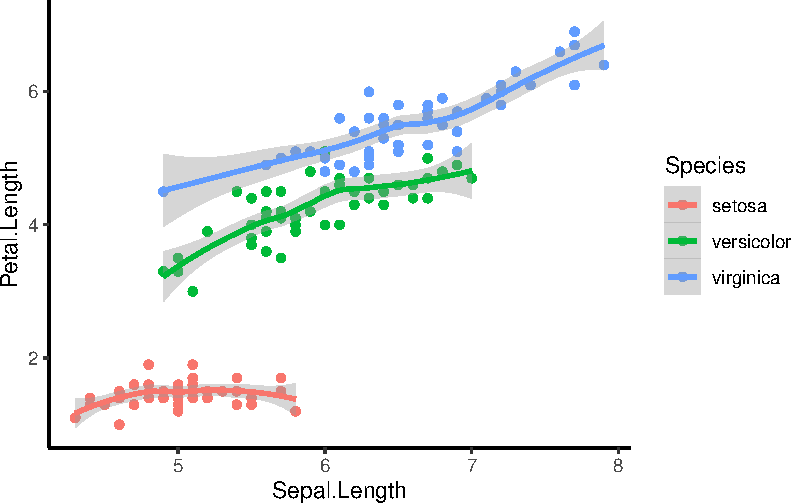
\includegraphics{quarto_basics_files/figure-pdf/unnamed-chunk-1-1.pdf}

}

\end{figure}

\hypertarget{yaml}{%
\paragraph{\texorpdfstring{\ul{Yaml}}{Yaml}}\label{yaml}}

\begin{itemize}
\item
  TOC
\item
  Format - html \& pdf
\item
  code-fold
\item
\item
  docx
\end{itemize}

\hypertarget{github}{%
\paragraph{\texorpdfstring{\ul{Github}}{Github}}\label{github}}

\begin{itemize}
\item
  github tab
\item
  command line github
\end{itemize}



\end{document}
